% !TEX root = MAIN.tex

%\chapter{FAQAS usage methodology}
\chapter{FAQAS Usage Methodology}
\label{chapter:methodology}

FAQAS led to the development of a toolset that includes the following components:
\begin{itemize}
\item MASS (Mutation Analysis for Space Software), a tool that automatically executes code-driven mutation analysis. Code-driven mutation analysis consists of automatically generating mutants by altering the source code of the software under test. MASS implements a pipeline that makes it feasible in the context of space software.
\item DAMAt (DAta-driven Mutation Analysis with Tables), a tool that automatically executes data-driven mutation analysis. Data-driven mutation analysis is an approach newly defined within FAQAS, which, instead of mutating the implementation of the software under test, alters the data exchanged by software components. Data-driven mutation analysis enables the injection of faults that affect simulated components (e.g., sensors), which is not feasible with traditional, code-driven mutation analysis.
\item SEMuS (Symbolic Execution-based MUtant analysis for Space software), a tool that automatically generates test inputs based on code-driven mutation analysis results.
\end{itemize}

\begin{figure}[tb]
\begin{center}
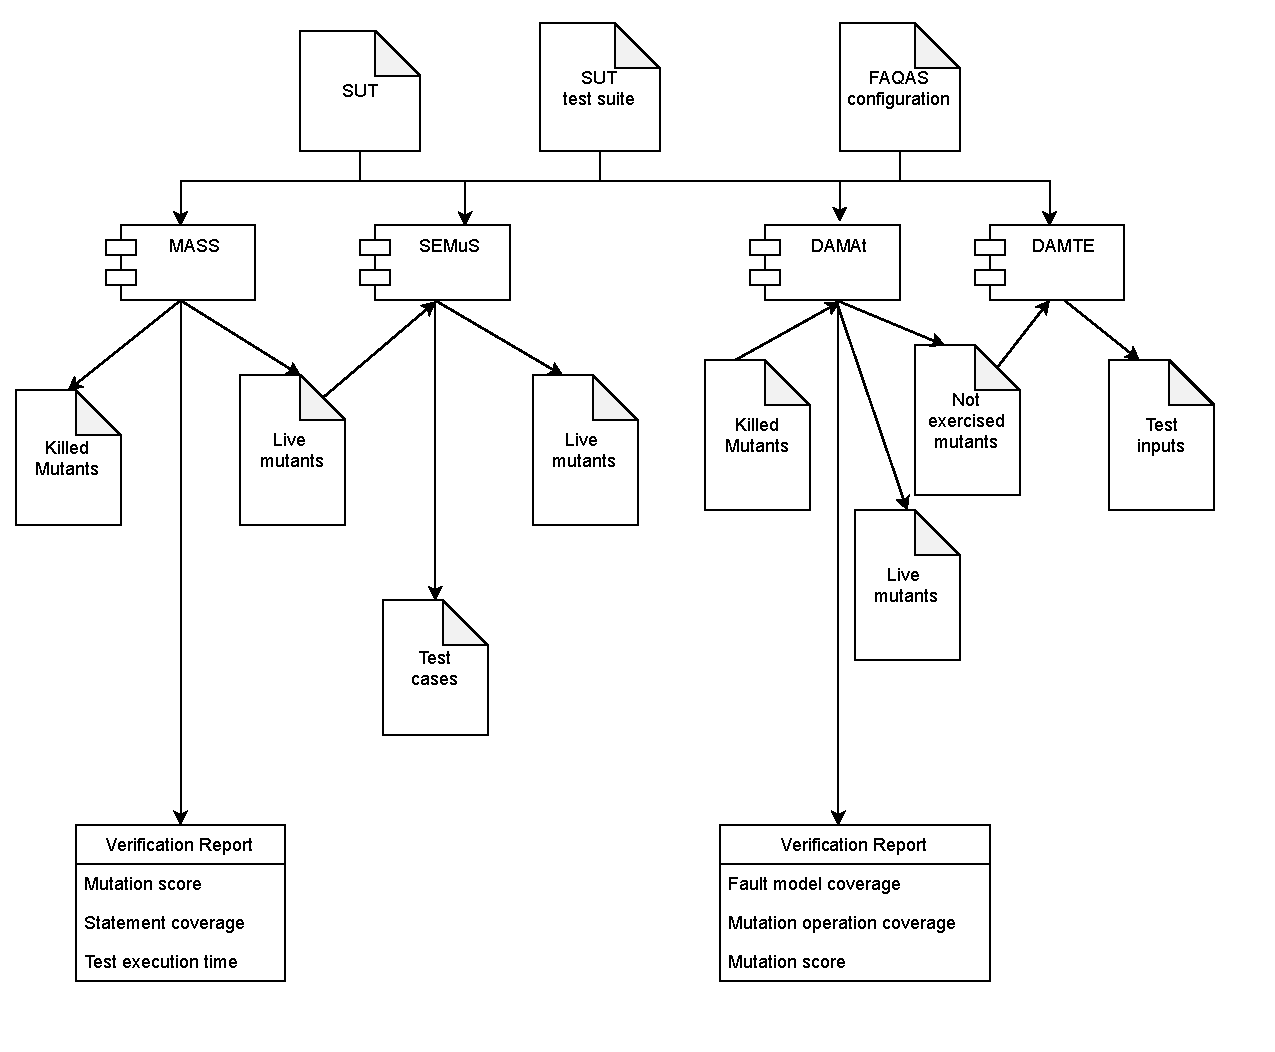
\includegraphics[width=0.8\textwidth]{images/FAQAS_drawio}
\caption{Overview of the FAQAS toolset}
\label{fig:FAQAS:toolset}
\end{center}
\end{figure}

The FAQAS activity also led to the definition and feasibility study of DAMTE, a methodology supported by the KLEE symbolic execution engine for the generation of test inputs based on data-driven mutation analysis results. However, DAMTE has shown to not be feasible in practice, with the current state-of-the-art test generation toolsets.

Figure~\ref{fig:FAQAS:toolset} provides an overview of the input and outputs of the FAQAS toolset. All the components take as input the software under test (SUT), its test suite, and a set of configuration files.
MASS generates as output a set of live mutants (i.e., mutants that do not lead to a test suite failure), a set of killed mutants (i.e., mutants that do not lead to a test suite failure), and information useful to draft a verification report, which includes the statement coverage of the SUT test suite, the mutation score, and the execution time of test cases.
SEMuS takes as input the list of live mutants detected by MASS and aims to generate test cases that kill them. After the
 execution of SEMuS, engineers have a set of additional test cases to be integrated into the SUT test suite and a list of live mutants (i.e., mutants for which SEMuS was not able to identify test inputs killing them). Live mutants shall be manually inspected by engineers to either determine if they are equivalent mutants or to manually derive a test input killing them.
 DAMAt generates as output a set of killed mutants (i.e., mutants that, during testing, successfully alter the data, and lead to test case failures), a set of live mutants (i.e., mutants that, during testing, successfully alter the data, but do not lead to test case failures), and a set of not executed mutants (i.e., mutants that, during testing, could not alter any data because the data they target is never exercised by the SUT); also, it provides information useful to draft a verification report, which includes the fault model coverage, the mutation operation coverage, and the mutation score.
 DAMTE is a manual procedure supported by the KLEE toolset that enables an engineer to automatically derive inputs that increase the fault model coverage and the mutation operation coverage.

In the following, we describe how the results generated by the FAQAS toolset enable the assessment and improvement of a test suite.
We focus on the fully automated tools, that is, MASS, DAMAt, and SEMuS.


\section{Code-driven Mutation Analysis: MASS}
\label{sec:meth:mass}

Code-driven Mutation Analysis shall be performed by applying the MASS toolset following the setup procedures described in the SUM. Figure~\ref{fig:MASS} provides an overview of the MASS workflow as presented in Section~\ref{sec:approach}. In addition it provides additional blocks, draw with dotted lines, showing how the MASS output might be used to improve the test suite. Also, we added the step \EMPH{Configure MASS} (i.e., \emph{Step 0}) to show the main configuration choices to be made by the engineer before running mutation analysis.

To run MASS, at a high-level, the engineer needs to make the following choices
\begin{itemize}
\item \EMPH{Select the source files to mutate}. Generally, all the source files of the SUT shall be considered for mutation. If the test suite targets only a subset  of files, the engineer can focus on that subset.
\item \EMPH{Select the sampling strategy}. If the test suite of the SUT takes more than one hour to be executed, we suggest to rely on the \emph{FSCI} mutant sampling strategy. Otherwise, engineers can execute all the mutants (i.e., set \emph{sampling=NO})
\item \EMPH{Enable test suite reduction and prioritization}. This choice enables MASS to further reduce test execution time by executing only a portion of the selected test cases based on statement coverage (see Section~\ref{sec:approach}). In case of system test suites testing an SUT with multiple tasks running in parallel we suggest to avoid reducing the test suite.
\end{itemize}

\STARTCHANGEDFINAL
% !TEX root =  ../MAIN.tex

\begin{table}[tb]
\footnotesize
\centering
\caption{\MASS minimal set of parameters to be configured.}
\label{table:to_configure}
\begin{tabular}{llp{7.5cm}}
\hline
\textbf{Script Name}  & \textbf{Parameter} &  \textbf{Description} \\
\hline
mass\_conf.sh & BUILD\_SYSTEM &  Specifies the building system type.\\
& PROJ &  Path of the SUT root  directory.\\
& PROJ\_SRC &  Path of the SUT source directory.\\
& PROJ\_TST &  Path of the SUT test  directory.\\
& PROJ\_COV &  Path of the directory with SUT coverage information.\\
& PROJ\_BUILD &  Path of the directory where the compiled binary is stored.\\
& ORIGINAL\_MAKEFILE &  Path to the original build script.\\
& COMPILATION\_CMD &  Compilation command of the SUT.\\
\hline
PrepareSUT.sh & None &  Commands shall be provided manually.\\
\hline
mutation\_additional\_functions.sh & run\_tst\_case  &  Implementation of the Bash function run\_tst\_case that executes the test case passed as a parameter.\\
\hline
\end{tabular}
\end{table}

In a nutshell the minimal set of parameters to be configured for MASS are listed and described in Table~\ref{table:to_configure}.
\ENDCHANGEDFINAL

For the other configuration choices for MASS, the default options are generally appropriate for most of the SUTs.

\begin{figure}[tb]
\begin{center}
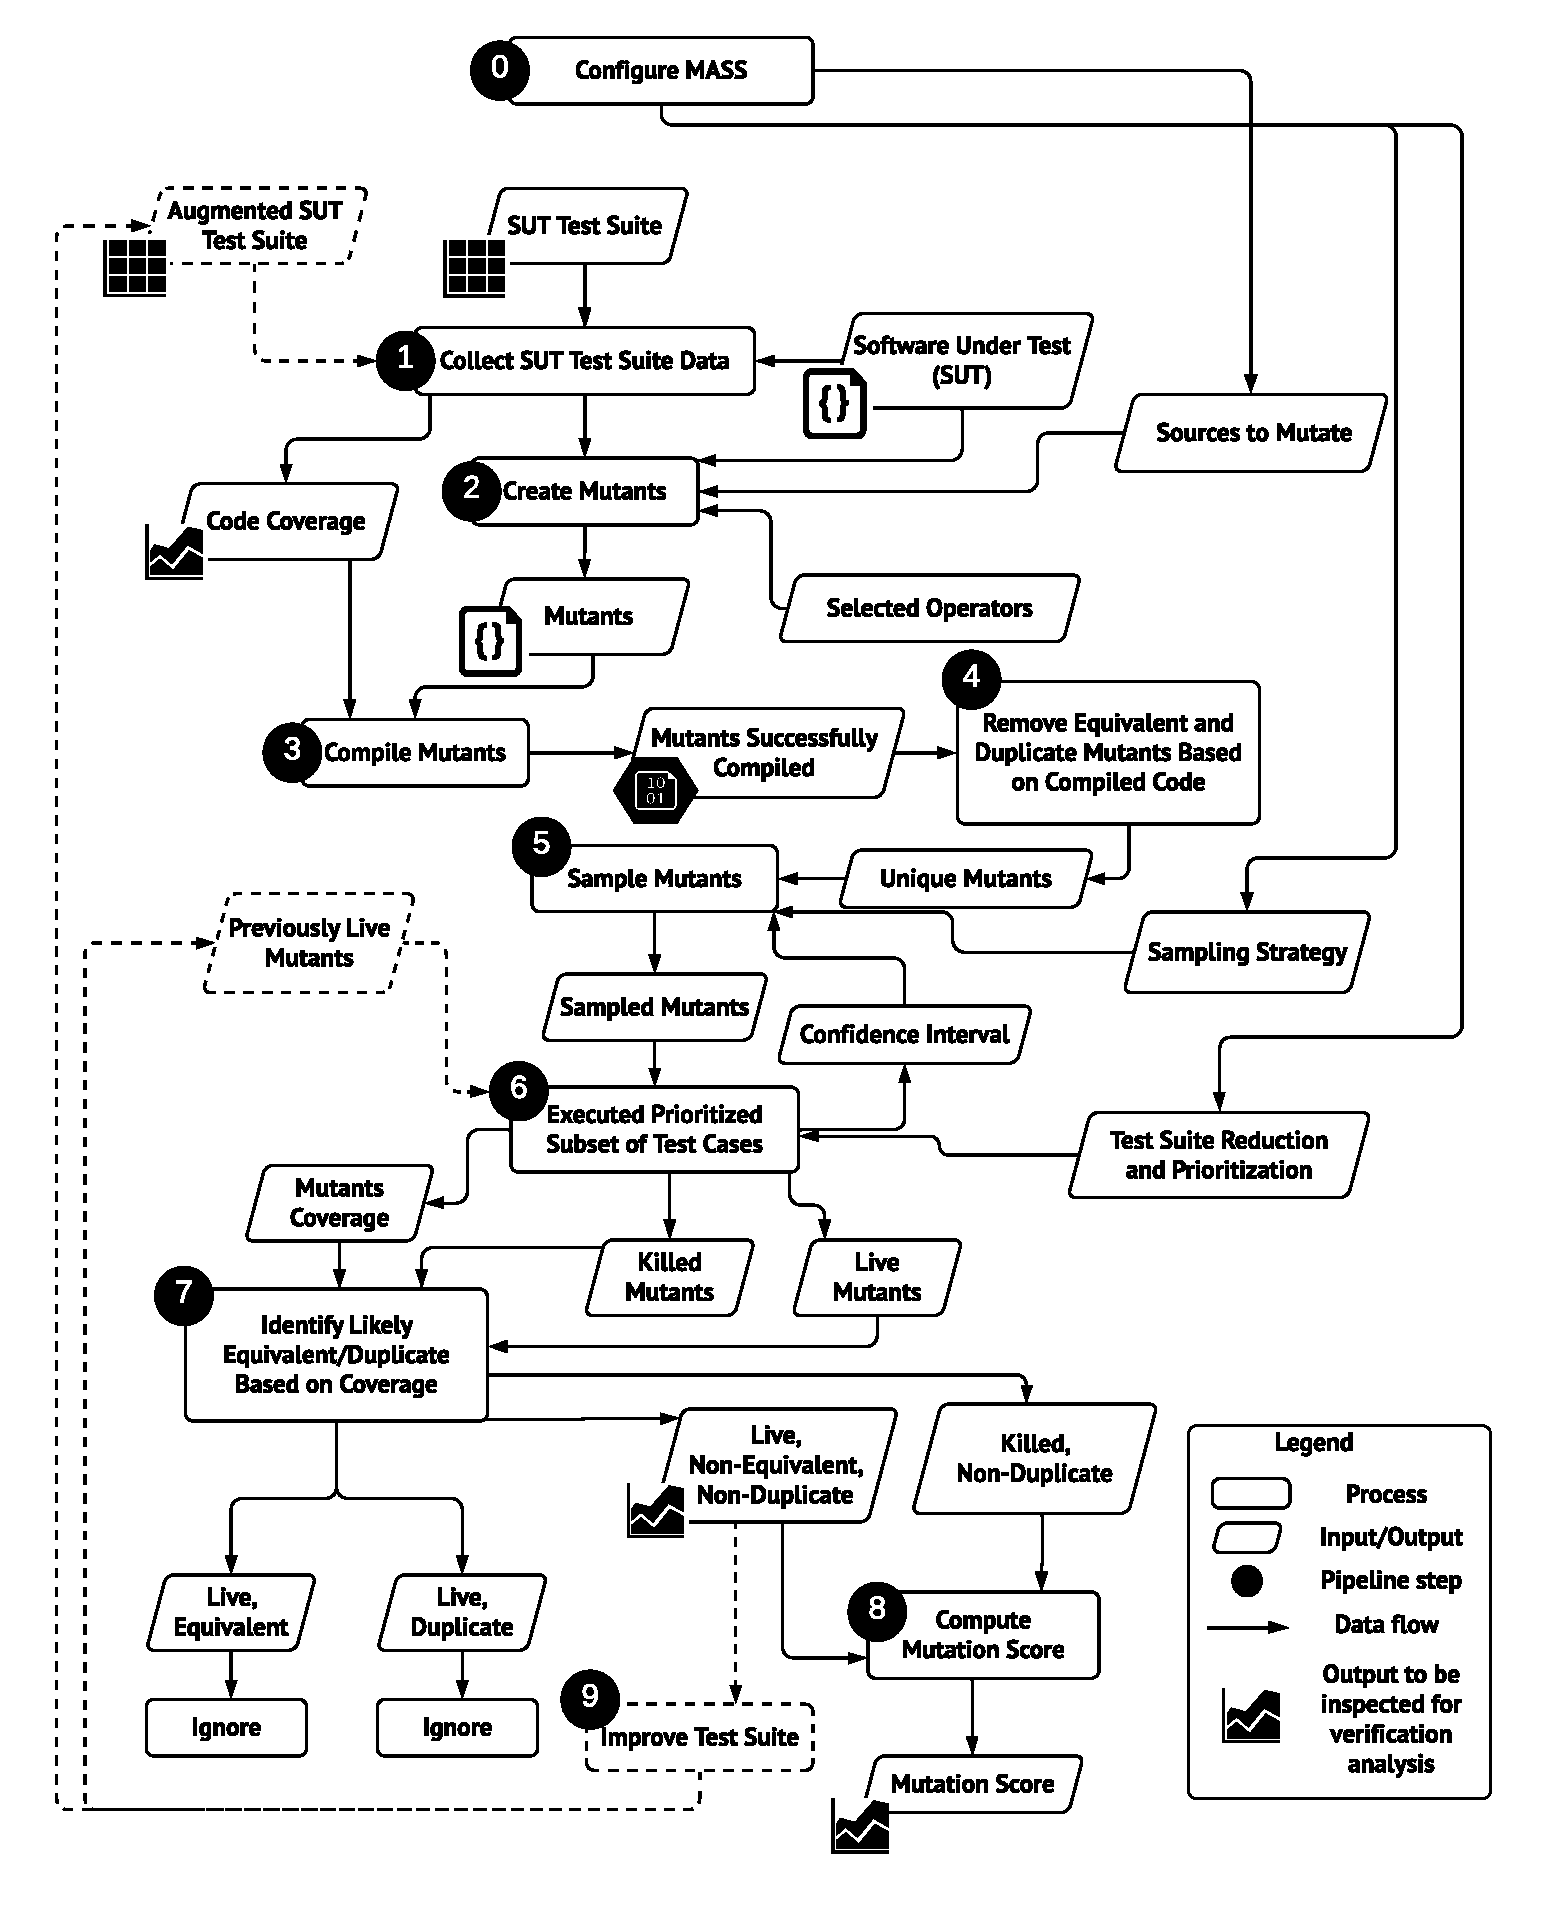
\includegraphics[width=0.8\textwidth]{images/MASS-extended.pdf}
\caption{Overview of the MASS workflow}
\label{fig:MASS}
\end{center}
\end{figure}



The main output of MASS is a file named \emph{MASS\_RESULTS}, which includes the metrics listed in Table~\ref{table:mass:metrics}.
Three additional relevant output files generated by MASS are \emph{filtered\_live}, \emph{useful\_list\_a} and \emph{useful\_list\_b}. They contain the names of the live mutants (i.e., the ones not killed by the test suite), they match the output box \emph{Live, Non-Equivalent, Non-Duplicate} in Figure~\ref{fig:MASS}.

\begin{table}[h]
\caption{MASS Metrics}
\label{table:mass:metrics}
\center
\begin{tabular}{|
@{\hspace{1pt}}p{120mm}|
}
\hline
\textbf{Metric name}\\
\hline
Number of mutants generated \\
%Mutants generation time&No\\
%Number of compiled mutants&No\\
%Percentage of compiled mutants&No\\
%Mutants compilation time&No\\
Number of mutants filtered using compiler optimisations \\
Sampling type \\
Number of mutants executed \\
%Number of test cases executed&No\\
%Test cases execution time \\
%Mutation execution traces \\
Number of killed mutants \\
Number of live mutants \\
Number of likely equivalent mutants \\
MASS mutation score \\
%List of useful mutants \\
Number of statements covered \\
Statement coverage \\
Minimum lines covered per source file \\
Maximum lines covered per source file \\
%Distribution of test cases exercising each statement&No\\
\hline
\end{tabular}
\end{table}

Within file \emph{MASS\_RESULTS}, the \EMPH{first metric} to be inspected is the \emph{Statement coverage} (i.e., the percentage of statements being covered). Since MASS generates mutants only for the statements being exercised by the test suite, a high mutation score in the presence of a low statement coverage cannot indicate that the test suite has high quality. In general, we assume that engineers apply MASS to test suites that have already achieved the required quality level, according to ECSS practice (e.g., statement coverage of 100\%). The statement coverage shall thus simply enable engineers to determine if the test suite is correctly executed through MASS (i.e., if the statement coverage generated by MASS matches the expected one). The statement coverage metric is also generated at the beginning of the mutation analysis process (i.e., Step 1 in Figure~\ref{fig:MASS}\footnote{Statement coverage information is provided in file \emph{coverage.txt.overall}.}); for this reason, in the case of low statement coverage, engineers can focus on improving the test suite without running the rest of the mutation analysis process. The \EMPH{second metric} to be inspected is the \emph{MASS mutation score}. It provides an indication of the quality of the test suite based on mutation analysis results. According to the literature on the topic,
%it shall be above 75\%, otherwise the test suite shall be improved by introducing additional test cases.
 achieving a high mutation score improves significantly the fault detection capability of a test suite~\cite{papadakis2018mutation}; also, a very high mutation score (i.e., above 0.75) ensures a higher fault detection rate than the one obtained with other coverage criteria, such as statement and branch coverage~\cite{Chekam:17}.


The next step is the \EMPH{improvement of the test suite}. This is performed by deriving test inputs that kill live mutants.
To this end, engineers shall inspect all the mutants appearing in the file \emph{useful\_list\_a}. For each mutant, the engineer shall implement a test case capable of killing the mutant (i.e., a test case that fails with the mutant but not with the original software).
The file \emph{useful\_list\_a} provides a list of mutants that are likely non redundant with each other because when tested by the SUT test suite they lead to a statement coverage profile (i.e., the set of statements covered during their execution) that differs.
The file \emph{useful\_list\_b} provides a list of mutants that are likely redundant with the ones appearing in the file \emph{useful\_list\_a}; therefore the mutants listed in the file \emph{useful\_list\_b} will be likely killed by test cases implemented to kill the mutants in \emph{useful\_list\_a}.
The mutants within file \emph{useful\_list\_a} are sorted according to their diversity (i.e., the mutants on top are likely very different from each other.
The file \emph{filtered\_live} provides the whole list of live mutants, that is the union of the mutants appearing in the files
\emph{useful\_list\_a} and \emph{useful\_list\_b}.

In general, since a same test case may kill more than one mutant, we suggest to derive test inputs for a subset of the mutants in \emph{useful\_list\_a} and then rerun the mutation analysis process. When rerunning the mutation analysis process, engineers shall focus the mutation analysis on the mutants appearing in \emph{useful\_list\_a} and in \emph{useful\_list\_b}. This is done by re-executing mutation analysis from step 6 (\emph{Execute mutants}), after replacing the mutant names in file \texttt{\$MASS\_WORKSPACE/COMPILED/all\_filtered} by the mutant names of list \emph{useful\_list\_a} and \emph{useful\_list\_b}.

When automated test generation with SEMuS is feasible; we suggest to rely on SEMuS to automatically generate test cases for all the mutants appearing in \emph{useful\_list\_a} and in \emph{useful\_list\_b} (see Section~\ref{sec:meth:semus}).

When identifying inputs that kill mutants (either manually or with SEMuS) engineers may detect equivalent mutants. Equivalent mutants shall be removed from the list of mutants considered for the analysis.

If mutation analysis has been performed through mutants sampling (e.g., with \emph{FSCI}), after test suite improvement (i.e., after introducing test cases that kill all the mutants in \emph{useful\_list\_a} and in \emph{useful\_list\_b}), it is necessary to re-run mutation analysis to estimate the mutation score for the whole system.

\clearpage
\section{Code-driven Mutation Testing: SEMuS}
\label{sec:meth:semus}

Figure~\ref{fig:semus_architecture_meth} provides the workflow of SEMuS; it has been described in Section~\ref{sec:semus}. The list of live mutants processed by SEMuS coincides with the list of mutants appearing in the file \emph{filtered\_live} presented in Section~\ref{sec:meth:mass}.

The mutants for which SEMuS does not generate a test case\footnote{In our toolset, such mutants are identifies by looking for empty folders within the output folder \emph{direct/TEMPLATE/FAQAS\_SEMu-out/produced-unittests}.} shall be manually inspected by engineers to determine if they are equivalent to the original software.

The test cases generated by SEMuS can instead be integrated as a regression test suite according to the \EMPH{test suite augmentation} procedure described in Section~\ref{sec:Semus:augment}. Otherwise, engineers can copy the source code of the generated test cases inside the test suite of the SUT and add assertions according to the expected output generated by SEMuS\footnote{Please recall that the output expected after the execution of a test case is written within a file with extension \emph{.expected}, as explained in Section~\ref{sec:Semus:augment}.}.

\begin{figure}[h]
\begin{center}
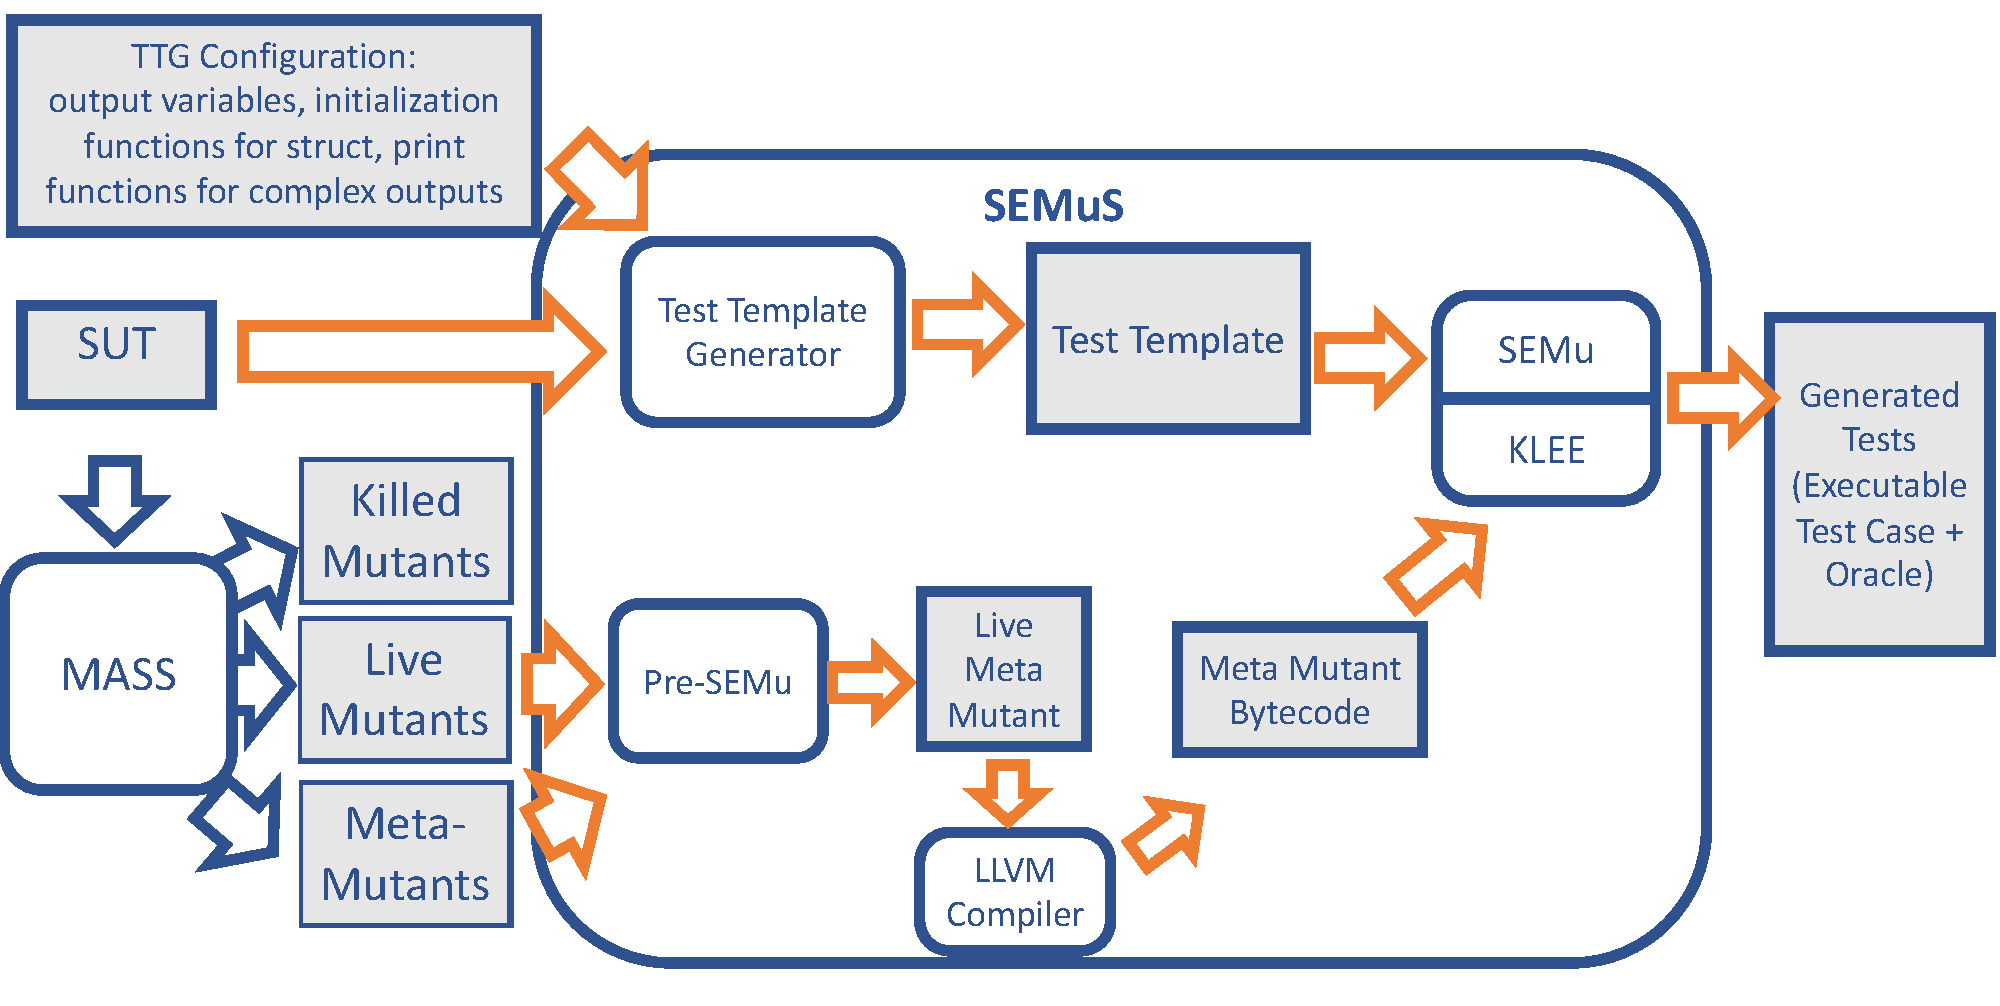
\includegraphics[width=0.8\textwidth]{images/semus-architecture2}
\caption{FAQAS-SEMuS Architecture and Workflow}
\label{fig:semus_architecture_meth}
\end{center}
\end{figure}

\clearpage
\section{Data-driven Mutation Analysis: DAMAt}
\label{sec:meth:damat}

DAMAt shall be configured and applied according to the procedure described in Section~\ref{sec:damat}.
After the execution, DAMAt generates two files: \emph{final\_mutants\_table.csv} and \emph{mutation\_sum\_up.csv}.
The latter provides a high-level perspective on the results of the procedure, because it contains the three metrics defined in Section~\ref{sec:mutationAnalysisResults}:
\begin{enumerate}
\item Fault model coverage, the percentage of fault models covered by the test suite.
\item Mutation operation coverage, the percentage of data items that have been mutated at least once, considering only those that belong to the data buffers covered by the test suite.
\item Mutation Score, the percentage of mutants killed by the test suite (i.e., leading to at least one test case failure) among the mutants that target a fault model and for which at least one mutation operation was successfully performed.
\end{enumerate}


A low score in one of the metrics indicate one of following scenarios, repsectively:
\begin{enumerate}
\item The message type targeted by a fault model is never exercised.
\item The message type is covered by the test suite, but it is not possible to perform some of the mutation operations. It depends on the fact that not all the input partitions are exercised by the test suite.
\item The mutation is performed but the test suite does not fail. It may depend on two reasons: (1) the test oracles are imprecise (e.g., they do not verify all the state variables), (2) the system is not brought into a state where the effect of the mutation is notices (i.e., the scenarios exercised are insufficient).
\end{enumerate}


 \begin{figure}[h]
\begin{center}
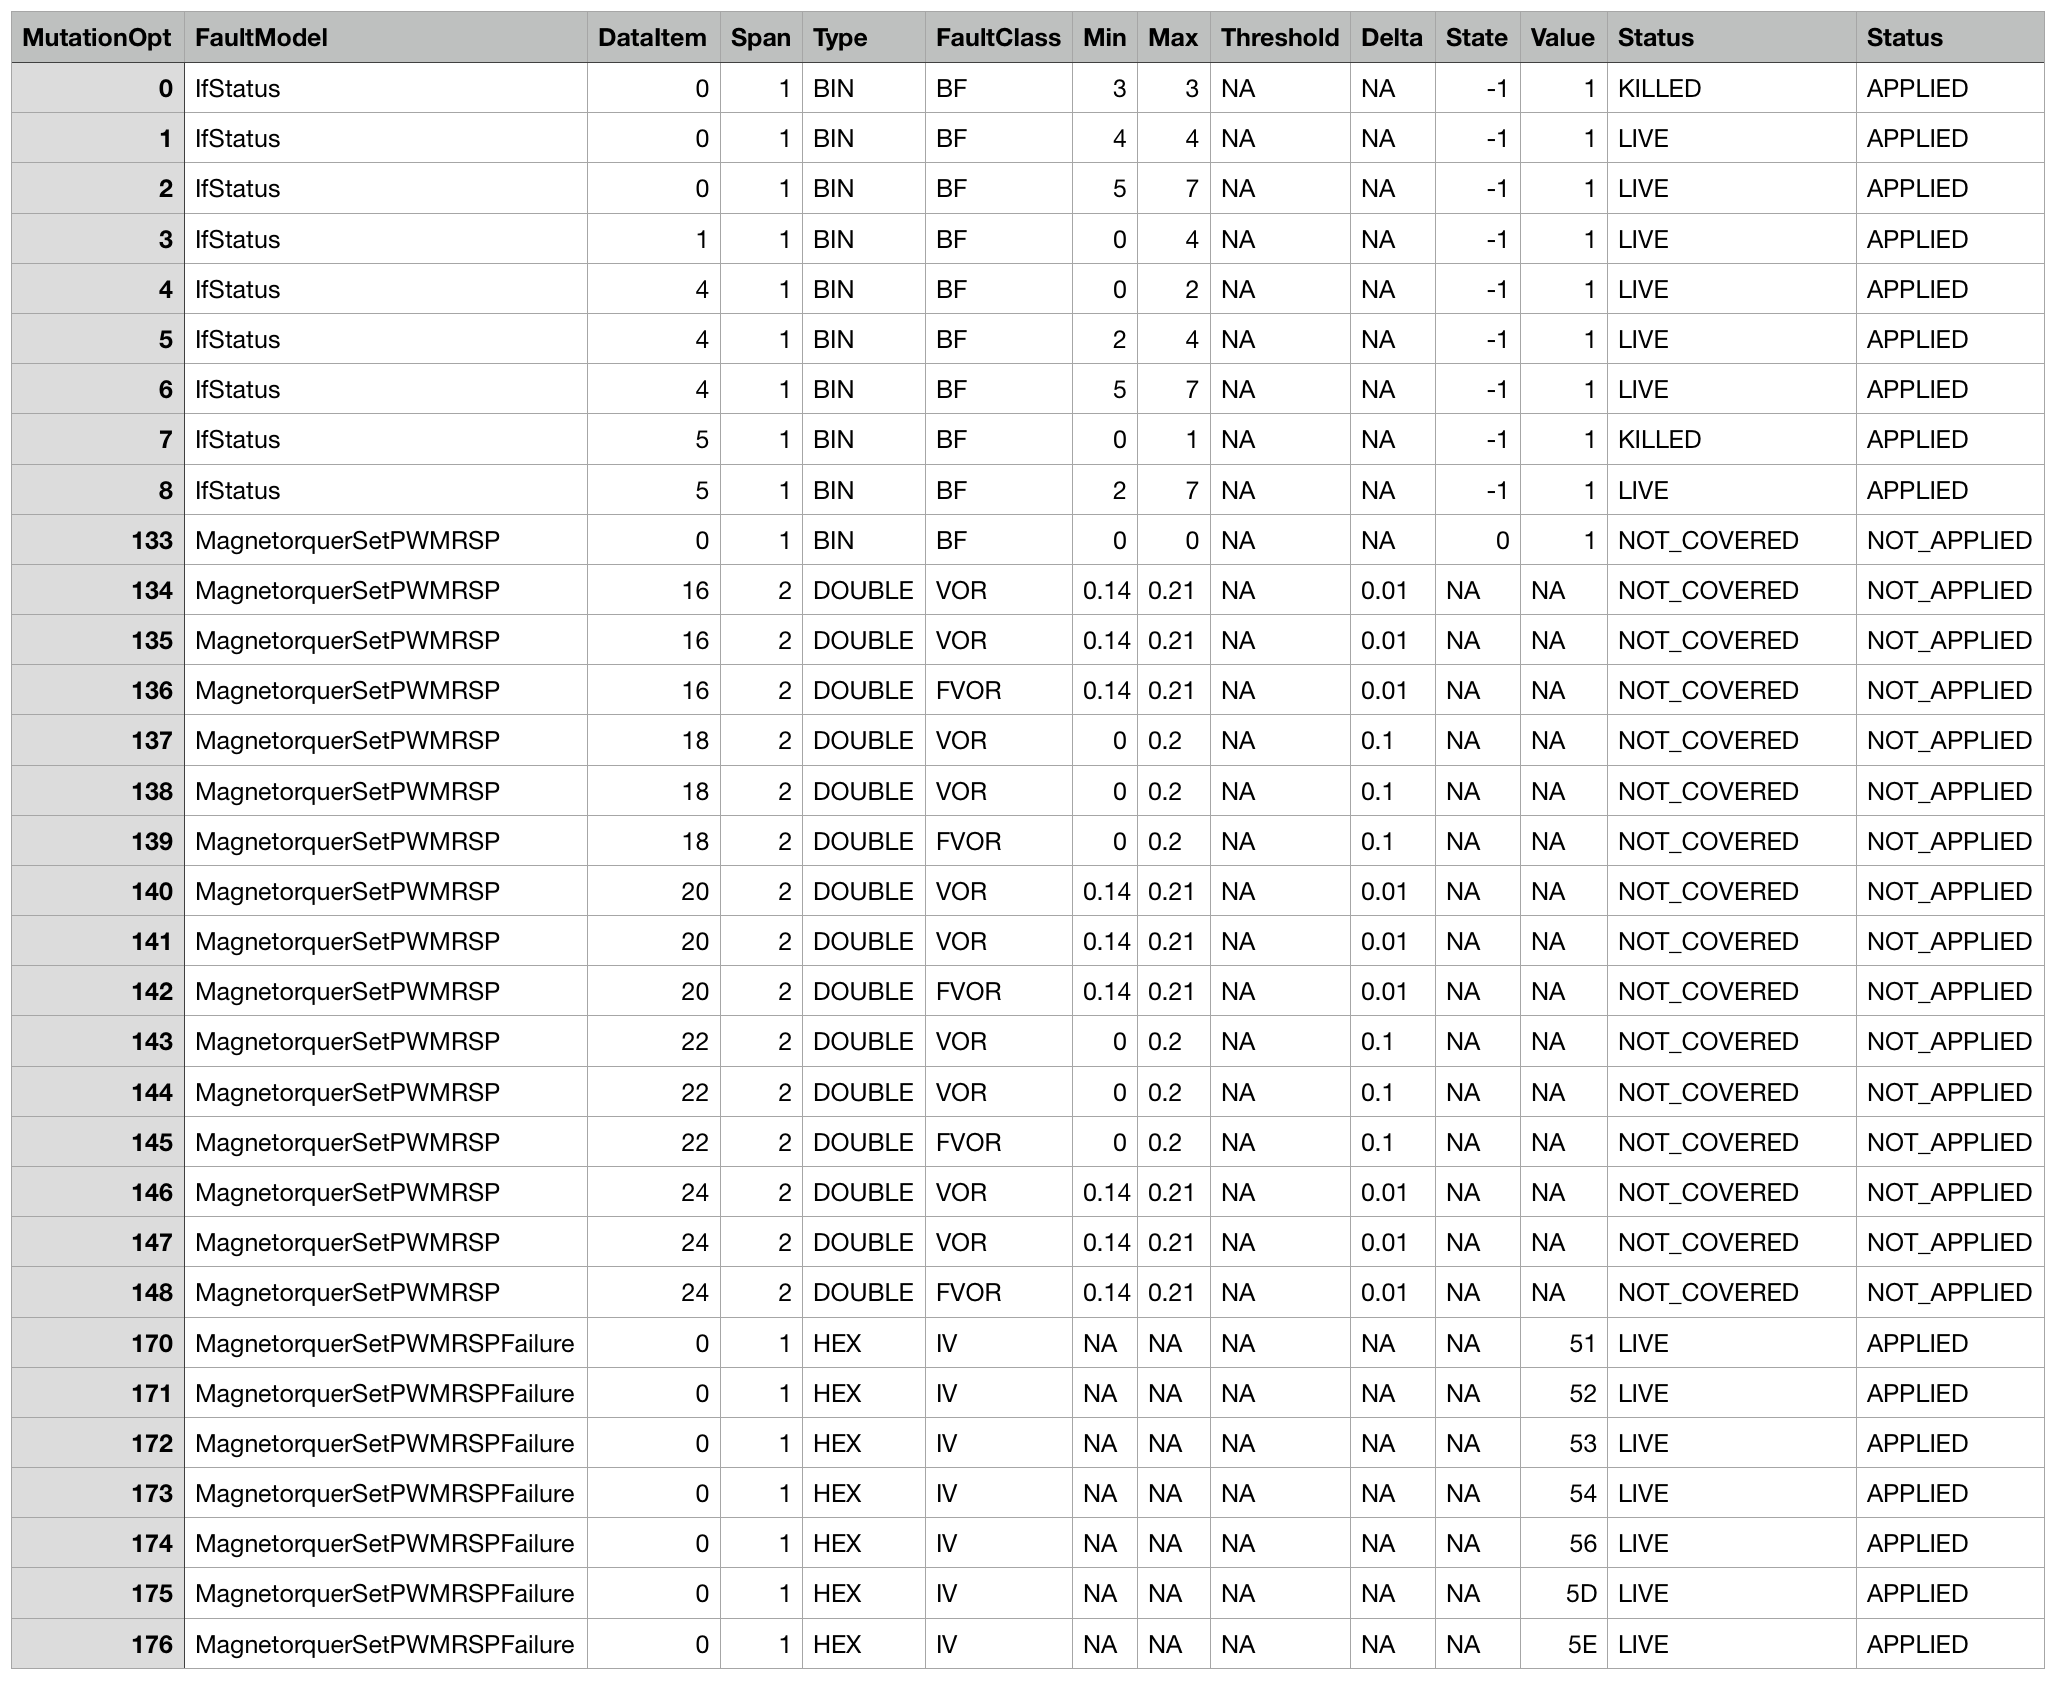
\includegraphics[width=0.8\textwidth]{images/DAMAtADCS.png}
\caption{DAMAt: Example of the result table \emph{final\_mutants\_table.csv}.}
\label{fig:damat:example:result:table}
\end{center}
\end{figure}

To determine how to improve the test suite, the engineer should look at the file \emph{final\_mutants\_table.csv}, which contains a summary of the results for each mutant. Figure~\ref{fig:damat:example:result:table} provides an excertp of the content of the cvs file generated for one of the case study subjects considered in our experiments, in tabular form. Column \emph{Status} reports about  the fault model coverage; indeed, mutants reported as \emph{NOT\_COVERED} indicate that the corresponding fault model is not covered by the test suite. Since we define a different fault model for each type of message exchanged by the software under test (e.g., each message may correspond to a different PUS command), the lack of coverage for a fault model indicates that a message type has not been exercised at all by the test suite. In practice this also means that the line of code where the mutation probe has been placed was not exercised.
To address such shortcoming, the the engineer shall define a test case that makes the SUT send that particular message type (or receive that particular message type).

The column named \emph{application} reports about the \emph{mutation operation coverage}. By looking at the mutants defined as \emph{NOT\_APPLIED} the engineer can determine if some input partitions (i.e., some subsets of the input range) had not been exercised by the test suite. Table~\ref{table:damat:interpretation} describes how to interpret the result reported in the Application column, for each type of mutant.
For example, if there is a Value Above Threshold that is not applied, this means that the particular data item targeted by the mutation was never below that threshold during the test suite execution.
This could give an insight on what kind of data is exchanged by the components during the execution to help determine if some use case is not considered in the test suite.


Last, by looking at what mutants remain LIVE after the execution of DAMAt, the user can identify cases in which the test suite does not fail although the data being exchanged is not the one expected by the engineer who wrote the test suite.
The simplest cause of such lack of failures is the absence of an oracle (or a poor oracle); for example, the test case assertions do not verify the output state of the SUT.
Another possibility is that the software reacts to the invalid data only when in a specific state; this means that the test suite lacks a test case in such a specific state.

For DAMAt, \EMPH{test suite augmentation} shall thus be performed manually by an engineer who shall define additional test cases based on the strategy reported above.

% !TEX root = ../MAIN.tex
\begin{table}[H]
\caption{Interpretation of results concerning the lack of coverage for mutation operations.}
\label{table:damat:interpretation}
\begin{tabular}{|p{2cm}|p{6cm}|p{6cm}|}
\hline
\textbf{Mutation Operator} & \textbf{If APPLIED} & \textbf{If NOT\_APPLIED} \\ \hline
\textbf{VAT} & The value of the targeted data item was below the threshold at least once. & The value of the targeted data item was never below the threshold. It indicates that the test suite does not cover the input partition (e.g., the test suite never tests the nominal case). \\ \hline
\textbf{VBT} & The value of the targeted data item was above the threshold at least once. & The value of the targeted data item was never above the threshold. It indicates that the test suite does not cover the input partition (e.g., the test suite never tests the nominal case). \\ \hline
\textbf{VOR} & The value of the targeted data item was inside the range defined by Min and Max at least once. & The value of the targeted data item was never observed within the range defined by Min and Max. It indicates that the test suite does not cover the min-max input partition (e.g., the test suite never tests the nominal case). \\ \hline
\textbf{BF} & At least a bit was flipped. If State was set to 1 this means that between Min and Max position at least a bit contained a 1. The same goes if State was set to 0. & No bits were flipped, this happens when the test suite never lead to the exchange of messages containing bits in the specified state (either $0$ or $1$). It indicates that an input partition is not covered.\\ \hline
\textbf{INV} & It is always applied.& It is always applied.\\ \hline
\textbf{IV} & The value of the targeted data item was different from the invalid value specified by the operator at least once.&
The value of the targeted data item was always equal to the invalid value specified by the operator at least once. It indicates that the test suite only test the software in the presence of a specific invalid value.\\ \hline
\textbf{ASA} & It is always applied.& It is always applied.\\ \hline
\textbf{SS} & It is always applied.& It is always applied.\\ \hline
\textbf{HV} & It is always applied.& It is always applied.\\ \hline
\textbf{FVAT} & The value of the targeted data item was above the threshold at least once. &
The value of the targeted data item was never above the threshold. It indicates that the test suite does not cover the input partition (e.g., it does not cover non-nominal cases).\\ \hline
\textbf{FVBT} & The value of the targeted data item was below the threshold at least once. & The value of the targeted data item was never below the threshold. It indicates that the test suite does not cover the input partition (e.g., it does not cover non-nominal cases).\\ \hline
\textbf{FVOR} & The value of the targeted data item was outside the range defined by Min and Max at least once. & The value of the targeted data item was never outside the range defined by Min and Max. It indicates that the test suite does not cover the input partition (e.g., it does not cover non-nominal cases). \\ \hline
\end{tabular}
\end{table}

